% \chapter*{Empirische Grundlagen} \label{empg}
% \section{Anforderungsmanagement}
% \footcite[Vgl.][o. S.]{Grande_2014_Anforderungsmanagement}


% Ziel des Anforderungsmanagements bzw. Requirements Engineerings nach Pohl und Rupp ist die Erfassung und Dokumentation von Anforderungen.\footcite[Vgl.][S. 3]{Pohl_2015_Requirements}
%
% Die Haupttätigkeiten sind die Ermittlung, Dokumentation, Prüfung und Verwaltung von Anforderungen, wobei die Verwaltung mit den drei vorigen Tätigkeiten einher geht. \footcite[Vgl.][S. 4 f.]{Pohl_2015_Requirements}
% %
% \subsection{Ermittlung}
% Bei der Ermittlung der Anforderungen werden verschiedene Quellen, wie z. B. Stakeholder, Dokumente oder aktive Systeme genutzt um Anforderungen zu detektieren und zu verfeinern.\footcite[Vgl.][S. 21]{Pohl_2015_Requirements}\\
% Das Interview ist eine mögliche Befragungstechnik, bei der ein Stakeholder (Interviewpartner) vom Requirements Engineer (Interviewer) vorgegebene Fragen gestellt bekommt. Die Antworten werden protokolliert. Etwaige Rückfragen können sofort im Gesprächsverlauf geklärt werden. Durch geschickt gestellte Fragen können auch unterbewusste Anforderungen ermittelt werden. Der Verlauf des Gesprächs kann individuell angepasst werden, es wird gezielt nachgefragt und auf einzelne Themen eingegangen, um das behandelte Thema möglichst komplett abzubilden.\footcite[Vgl.][S. 28]{Pohl_2015_Requirements}
%
% \subsection{Dokumentation}
% Die erarbeiteten Anforderungen werden in natürlicher Sprache oder in dafür vorgesehenen Modellen dokumentiert, wobei entsprechende Techniken zum Einsatz kommen. \footcite[Vgl.][S. 4]{Pohl_2015_Requirements}\\
% Die im Requirements Engineering anfallenden Tätigkeiten müssen geeignet dokumentiert werden. Dazu zählt z. B. auch die Erstellung von Interviewprotokollen. Als Dokumentation gilt jede Form der formalen Darstellung, von Beschreibung in natürlicher über strukturierten Text bis hin zu formalen Techniken wie Diagrammen. Die Dokumentationsform sollte der zugrundeliegenden Aktivität angemessen sein und diese sinnvoll wiedergeben. \footcite[Vgl.][S. 35 ff.]{Pohl_2015_Requirements}

% \subsection{Prüfung}
% % Um die Qualität der Anforderungen gewährleisten zu können, muss diese frühzeitig geprüft werden.\footcite[Vgl.][S. 4]{Pohl_2015_Requirements}
% Zu den Qualitätskriterien zählen u.A. Korrektheit und Abgestimmtheit. Die Methoden der Qualitätskontrolle können dabei sowohl für einzelne Anforderungen, als auch für Anforderungsdokumente eingesetzt werden.
% Bei der Überprüfung der Anforderungen sollen Fehler wie \glqq{}Mehrdeutigkeit, Unvollständigkeit und Widersprüche\grqq\footcite[][S. 95]{Pohl_2015_Requirements} aufgedeckt werden.\footcite[Vgl.][S. 95]{Pohl_2015_Requirements}

\subsection{Verwaltung}
Die Verwaltung der Anforderungen erfolgt parallel zu den vorher genannten Tätigkeiten und beinhaltet die Strukturierung und Aufbereitung für verschiedene Rollen.\footcite[Vgl.][S. 5]{Pohl_2015_Requirements}\\
Außerdem werden Verfolgbarkeit, Versionierung, Priorisierung und die Verwaltung von Änderungen unter Beibehaltung der Konsistenz sichergestellt. Auch hier reicht der Fokus von Einzelanforderungen bis hin zu Anforderungskatalogen.
Die Anforderungen werden mit den Informationen Identifikator, Name, Autor und Quelle versehen. Die Priorisierung der Anforderungen kann z. B. durch den Auftraggeber oder Faktoren wie die Dringlichkeit der Umsetzung geschehen.\footcite[Vgl.][S. 126]{Pohl_2015_Requirements}

% \section{Qualitative Inhaltsanalyse}
% \footcite[Vgl.][S.]{Mayring_2009_qualitative_Inhaltsanalyse}

% \todo{Systematisierendes Interviews --> Qualitative Inhaltsanalyse}
% \question{Muss ich die qualitative Inhaltsanalyse erläutern oder reicht das Experteninterview?}

Die qualitative Inhaltsanalyse nach Mayring ist eine Technik zur Auswertung und Interpretation von Text. Sie kann als eigenständige Erhebungsmethode betrachtet werden und hat zum Ziel, Kategorien aus Textbestandteilen zu bilden und den Inhalt sinngemäß zusammenzufassen. \footcite[Vgl.][S. 671]{Mayring_2009_qualitative_Inhaltsanalyse}\\
Das Experteninterview ist eine Möglichkeit, die qualitative Inhaltsanalyse durchzuführen und beinhaltet u.a. Audioaufnahme und Transkription.\footcite[Vgl.][S. 673 f.]{Mayring_2009_qualitative_Inhaltsanalyse}

In dieser Arbeit wird das Experteninterview als spezielle Form der qualitativen Inhaltsanalyse verwendet. Auf eine Detailbeschreibung dieser wird daher verzichtet und das Experteninterview dafür in \autoref{Experteninterview} ausführlich beschrieben.

% \section{Experteninterview} \label{Experteninterview}
Heutzutage ist die Bedeutung von Experteninterviews in der Forschungspraxis unumstritten. In verschiedensten Bereichen gehört es fest zum Kernbestand der alltäglichen Forschungsroutine, sei es als eigenständige Erhebungsmethode oder als ergänzende Methode im Rahmen explorativer Forschung. \footcite[Vgl.][S. 1]{Bogner_2014_Interview}

% Wesentliche Funktionen des Experteninterviews sind Informationsgewinnung und Theorieentwicklung, weswegen es sich als Methode eignet, um Anforderungen zu erheben.
% \footcite[Vgl.][S. 187 f.]{Glaeser_2010_Inhaltsanalyse}$^,$\footcite[Vgl.][S. 9]{Bogner_2014_Interview}
%
% Wenn von Experteninterviews die Rede ist, kann man davon ausgehen, dass ein leitfadengestütztes, qualitatives Interview gemeint ist. Da das Instrument Experteninterview dem Forschungsvorhaben angepasst werden muss, können jedoch verschiedene Dinge unter dem Begriff verstanden werden und es ist nötig klarzustellen, welche Ausprägung gemeint ist.\footcite[Vgl.][S. 3]{Bogner_2014_Interview}
% Auch der Expertenbegriff muss der Forschungsfrage angepasst werden.\footcite[Vgl.][S. 180]{Meuser_1994_Interview}

% In dieser Arbeit wird ausschließlich der qualitativ ausgerichtete Ansatz von Meuser und Nagel verfolgt. Quantitative Ansätze oder qualitative Ansätze anderer Autoren, die von dem behandelten abweichen werden hier nicht weiter ausgeführt.\footcite[Vgl.][o.S.]{Meuser_2010_Interview}

% Um das Experteninterview anwenden zu können, muss geklärt werden, wer als Experte gilt, was Expertenwissen bedeutet und wie man es abruft, welche Schritte zur Vorbereitung eines Interviews erforderlich sind, welche Gesprächsführung für die Forschungsfrage Sinn macht und wie die Interviews ausgewertet werden können.\footcite[Vgl.][S. 6 f.]{Bogner_2014_Interview}


% \subsection{Arten}
% Meuser und Nagel unterscheiden Experteninterviews grundlegend in systematisierende und explorativ-felderschließende Interviews. Bei ersteren wird der Experte zu seinem eigenen Fachgebiet befragt (Betriebswissen), bei letzerem liefert er lediglich \glqq{}Informationen über die Kontextbedingungen des Handelns der Zielgruppe\grqq (Kontextwissen)\footcite[][S.445]{Meuser_1991_Interview} .
%
% Bogner, Littig und Menz sprechen in diesem Zusammenhang von fundierenden und explorativen Interviews und fasst die vormals genannten Kategorien unter dem Begriff \textit{informatorisch} zusammen. Außerdem ergänzt er zwei  deutungswissenorientierten Varianten. Eine genaue Aufschlüsselung ist in \autoref{tab:artenei} zu sehen.\footcite[Vgl.][S. 445 f.]{Meuser_1991_Interview}$^,$\footcite[Vgl.][S. 22 ff.]{Bogner_2014_Interview}
%
%
% \begin{table}[H]
% \centering
% \begin{tabularx}{1\textwidth}{XXX}%
%                             & Explorativ (Kontextwissen) & Fundierend (Betriebswissen) \\\midrule
%    Informatorisch           & Explorative Datensammlung & Systematisierendes Interview \\
%    Deutungswissenorientiert & Exploration von Deutungen & Theoriegenerierendes Interview
% \end{tabularx}
%   \\\quelle{Bogner_2014_Interview}
%   \\\quelle{Meuser_1991_Interview}
% \caption{Arten von Experteninterviews}
% \label{tab:artenei}
% \end{table}


\subsection{Phasen}
% Ein Experteninterview kann aus bis zu acht Phasen bestehen, diese sind in \autoref{tab:phasenei} aufgeführt und anschließend im Detail erläutert. Für die Abfrage von Betriebswissen müssen alles Phasen durchlaufen werden, bei Kontextwissen entfallen die letzten beiden.\footcite[Vgl.][S. 466 f.]{Meuser_1991_Interview}

\begin{table}[ht]
\centering
\begin{tabularx}{1\textwidth}{llX}%
Nr. & Phase                            & Aktivitäten \\\midrule
1   & Leitfadenerstellung              & Erstellung des Leitfadens\\
2   & Tonaufnahme                      & Aufzeichnung des Gesprächs\\
3   & Transkription                    & Übertragung in Schriftdeutsch\\
4   & Paraphrase                       & Zusammenfassung und thematische Einteilung\\
5   & Überschriften                    & Verdichtung, Betitelung der paraphrasierten Abschnitte\\
6   & Thematischer Vergleich           & Vergleich aller Intervews, Suche nach Gemeinsamkeiten\\
7   & Soziologische Konzeptualisierung & Systematisierung, Typisierung, Deutung \\
8   & Theoretische Generalisierung     & Bildung von Theorien, Interpretation der Ergebnisse
\end{tabularx}
  \\\quelle{Meuser_1991_Interview}
\caption{Phasen eines Experteninterviews}
\label{tab:phasenei}
\end{table}

% \subsubsection{Transkription}
% Das Hauptaugenmerk von Experteninterviews liegt auf der Gewinnung von Wissen. Daher ist eine mühselige Notation, wie sie bei narrativen Interviews vorgenommen wird nicht nötig. Elemente wie Pausen, Betonung oder Stimmlage werden nicht interpretiert.
% Eine Transkription wird in der Regel nicht für die gesamte Tonaufnahme durchgeführt, sondern kann selektiv erfolgen. Bei der Abfrage von Betriebswissen fällt die Transkription umfangreicher aus als bei Kontextwissen. \footcite[Vgl.][S. 455 f.]{Meuser_1991_Interview}
%
% \subsubsection{Paraphrase}
% Die Paraphrase erfolgt unter Berücksichtigung der Forschungsfrage und gibt die Aussagen der Experten chronologisch geordnet und unverfälscht wieder, wobei diese zu thematischen Verbünden zusmamengefasst werden. Ob die Passage zusammenfassend oder detailliert wiedergegeben wird hängt von der Priorität des Themas und nicht zwangsläufig von der ihm gewidmeten Zeit ab.\footcite[Vgl.][S. 456 f.]{Meuser_1991_Interview}
%
% \subsubsection{Überschriften}
% Die paraphrasierten Abschnitte werden möglichst textnah mit einer oder mehreren Überschriften versehen, je nach dem, wie viele Themen angesprochen werden. Dabei ist darauf zu achten, dass das Expertenwissen im Fokus steht, der Experte als Person ist nicht relevant.\footcite[Vgl.][S. 458 f.]{Meuser_1991_Interview}

% \subsubsection{Thematischer Vergleich}
% Ab diesem Schritt werden nicht mehr die Interviews im Einzelnen betrachtet, es erfolgt ein Vergleich der thematisch ähnlichen Textpassagen aller Interviews, wobei die Überschriften nach Möglichkeit vereinheitlicht werden. Es wird geprüft, ob sich die Äußerungen der Experten decken oder ob sie unterschiedliche Ansichten haben. Außerdem wird betrachtet, zu welchen Themen sich alle Experten äußern und zu welchen nur einzelne.\footcite[Vgl.][S. 459 f.]{Meuser_1991_Interview}$^,$\footcite[Vgl.][S. 37]{Matthes_1986}
%
\subsubsection{Soziologische Konzeptualisierung}
In diesem Schritt werden aus dem gemeinsamen Wissen der Experten Kategorien gebildet, wodurch eine weitere Verdichtung des Wissens erfolgt. Dadurch soll eine Typisierung, Verallgemeinerung und Deutung des Wissens möglich werden. Die Struktur des Expertenwissens wird betrachtet, wodurch die Reichweite der Konzepte geprüft werden kann.\footcite[Vgl.][S. 462 f.]{Meuser_1991_Interview}

\subsubsection{Theoretische Generalisierung}
Im letzten Schritt werden Theorien aus Sinnzusammenhängen gebildet und die Ergebnisse interpretiert, wobei darauf zu achten ist, dass man sich nicht von Verdachten leiten lässt, sonder nur mit dem Forschungsmaterial arbeitet.\footcite[Vgl.][S. 463 ff.]{Meuser_1991_Interview}




\subsection{Definition: Experte}
% Das Wort \textit{Experte} leitet sich aus dem lateinischen \textit{expertus} (erprobt, bewährt) ab, welches wiederum aus dem passiven Verb \textit{experiri} (prüfen, ausprobieren) gebildet wird. Experten sind also Fachleute und Kenner, bzw. allgemein gesprochen Personen, die über ein gewisses Spezialwissen verfügen, das auf der Erfahrung des ausgiebigen Prüfens und Ausprobierens fußt. \footcite[Vgl.][S. 9]{Bogner_2014_Interview}
%
% Wie in \autoref{fig:experte} zu erkennen, zeichnet sich ein Experte durch eine bestimmte Kombination von Macht und Wissen aus, welche ihn von Eliten, Spezialisten und spezialisierten Laien unterscheidet.\\ \glqq{}Der Experte ist -- im Gegensatz zum Spezialisten – nicht allein durch Sonderwissen in Form fachspezifischer Kompetenzen charakterisiert, sondern durch seine Fähigkeit, Verbindungen zu anderen Wissensbeständen und Wissensformen herzustellen und die Relevanz des eigenen Wissens zu reflektieren\grqq. \footcite[][S. 14]{Bogner_2014_Interview}$^,$\footcite[Vgl.][S. 21 f.]{Hitzler_1994}
%
% \begin{figure}[H]
%   \centering
%   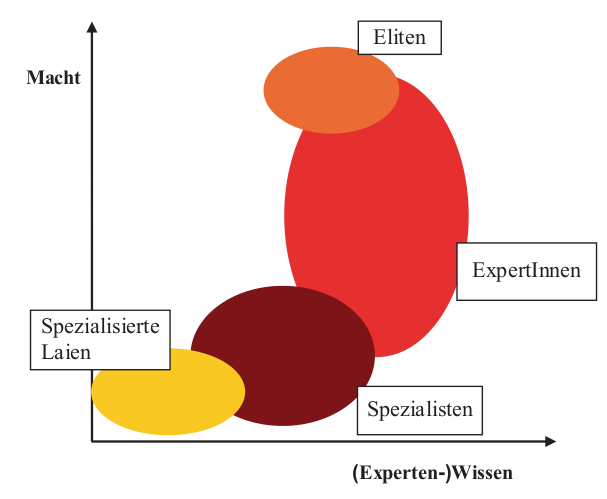
\includegraphics[width=0.6\textwidth]{Anhang/Experte}
%   \\\quelle{Littig_2008}
%   \caption{Experteneinordnung}
% \label{fig:experte}
% \end{figure}
%
% Gläser und Laudel definieren Experten als Menschen, die ein besonderes Wissen über soziale Sachverhalte besitzen.\footcite[Vgl.][S. 12]{Glaeser_2010_Inhaltsanalyse} Man könnte nun davon ausgehen, dass jeder ein Experte ist, da er sich in seinem Fachgebiet gut auskennt. Genauer betrachtet  gibt es jedoch große Unterschiede zwischen Laien und Experten, man bedenke nur das Verhältnis zwischen Ärzten und Patienten. Ein solcher Expertenbegriff ist also zu weit gefasst und es kann nicht jedes qualitative Interview automatisch als Experteninterview bezeichnet werden.\footcite[Vgl.][S. 10 f.]{Bogner_2014_Interview}
%
% Meuser und Nagel hingegen betrachten den Experten als Konstrukt des Forschungsinteresses. Die Expertise ist also keine allgemeingültige Eigenschaft oder Fähigkeit einer Person, sondern eine Zuschreibung des Forschenden an diese, im speziellen Kontext der Forschungsfrage. \footcite[Vgl.][S. 181]{Meuser_1994_Interview}
%


\subsection{Definition: Expertenwissen}
Als einer der ersten hat Schütz das Expertenwissen als sicheres und eindeutiges Wissen beschrieben, das dem Experten \glqq{}jederzeit kommunikativ und reflexiv\grqq\footcite[][S. 12]{Bogner_2014_Interview} verfügbar ist.\footcite[Vgl.][S. 86 ff. ]{Schuetz_1972}
Sprondel ergänzte anschließend, dass das Expertenwissen komplex integrierte Wissensbestände umfasst und auf den professionellen Funktionskontext bezogen ist.\footcite[Vgl.][S. ]{Sprondel_1979}

Expertenwissen spielt in der modernen Gesellschaft eine wichtige Rolle in allen Lebensbereichen, nicht nur in der Wissenschaft. Z. B. Fragen der Gesundheit oder Ernährung werden nicht intuitiv entschieden, sondern auf Basis von Expertise. Dieser Umstand stellt zwar eine Abhängigkeit dar, trägt jedoch dazu bei, dass unsere heutige Gesellschaft eine Wissensgesellschaft mit starker Spezialisierung ist.\footcite[Vgl.][o.S.]{Coser_1992}$^,$\footcite[Vgl.][S. 10]{Bogner_2014_Interview}
% \todo{Seite suchen: Giddens1991}
Umgekehrt betrachtet stellte Nowotny fest, dass die Expertise heutzutage nicht nur in der Wissenschaft, sondern in allen Bereichen der Gesellschaft gebildet wird.\footcite[Vgl.][S. 215 ff. ]{Nowotny_2001}$^,$\footcite[Vgl.][S. 10]{Bogner_2014_Interview}
%
% Das Interessante am Expertenwissen ist nicht nur das Wissen an sich, sondern die Wirkung in der Praxis. Experten werden gefragt, weil ihre Entscheidungen und Ratschläge das Handeln anderer Akteure mitstrukturieren und -gestalten.\footcite[Vgl.][S. 13]{Bogner_2014_Interview} Bogner spricht davon, dass Expertenwissen \glqq seine Bedutung über [...] soziale Wirkmächtigkeit\grqq{} erhält.\footcite[][S. 13]{Bogner_2014_Interview}
% Ferner folgert er daraus die Definition:\\ \glqq Experten lassen sich als Personen verstehen, die sich -- ausgehend von einem spezifischen Praxis- oder Erfahrungswissen, das sich auf einen klar begrenzbaren Problemkreis bezieht -- die Möglichkeit geschaffen haben, mit ihren Deutungen das konkrete Handlungsfeld sinnhaft und handlungsleitend für Andere zu strukturieren.\grqq{}\footcite[][S. 13]{Bogner_2014_Interview}
%

% \subsection{Vorbereitung des Interviews}
%   \todo{Erstellung des Leitfadens}
% \subsection{Wahl der Gesprächsführung}
% \subsection{Auswertung der Interviews}
%
% \footcite[Vgl.][S. 448 f.]{Meuser_1991_Interview}
%   \todo{Auswertung, Transkription, Paraphrase, Überschriften, Theoretischer Vergleich,}
%

% \footcite[Vgl.][o. S.]{Burger_2011_Interview}



\chapter{Grundlagen} \label{theg}
\section{Chatbots}
Ein Chatbot ist ein Programm, das für den Dialog mit Menschen erdacht ist und natürliche Sprache als Text oder Audio entgegennehmen und verarbeiten kann.
Chatbots werden hauptsächlich auf Websites und Instant-Messaging Systemen eingesetzt.
Benutzereingaben werden angenommen und passende Antworten dazu ausgegeben. Außerdem sollen Chatbots Gäste begrüßen und die Unterhaltung in Gang halten.\\
Chatbots können rein regelbasiert oder \acf{KI}-gesteuert reagieren.\\
Durch die inhärente Automatisierung sind Chatbots relevant bezüglich der \glqq{}Unterstützung und Ersetzung von Arbeitskräften\grqq
\footcite[][o. \pno]{Bendel_2018_Chatbot_Definition}{}.
\footcite[Vgl.][o. \pno]{Bendel_2018_Chatbot_Definition}

Chatbots können mit realen Personen oder anderen Chatbots kommunizieren. Ein Chatbot ist jeweils für einen bestimmten Aufgabenbereich vorgesehen und deckt nicht das gesamte Spektrum der menschlichen Kommunikation ab. Ähnlich wie bei Avataren können Chatbots eine \glqq{}körperliche Erscheinung\grqq
\footcite[][71\psq]{de_Vries_2006}
und \glqq{}virtuelle Identität\grqq
\footcite[][71\psq]{de_Vries_2006}
bzw. Charakter haben.
\footcite[Vgl.][71\psq]{de_Vries_2006}

Im Gegensatz zu Agenten arbeiten Chatbots nicht autonom, sondern reaktiv. Sie sind also auf die Befehle von Menschen angewiesen.
\footcite[Vgl.][69\psqq]{de_Vries_2006}

Entscheidend für die Gesprächskompetenz von Chatbots ist das zugrundel iegende Wissen. Die eingesetzten Algorithmen spielen nur eine nachgelagerte Rolle.\\
Für komplexere Problemstellungen  kann es nötig werden, den Kontext genauer zu erfassen. Dazu kann die Gesprächshistorie berücksichtigt und Laufzeitvariablen pro Nutzer gespeichert werden.
\footcite[Vgl.][82\psq]{Feindt_2006_Agenten}

\subsection{Komponenten}
Die wesentlichen Komponenten eines Chatbots sind Utterances (Äußerungen), Intents (Absichten) und Entities (Entitäten).\\
Als Äußerungen gelten alle Eingaben des Nutzers in ihrer Basisausprägung, z. B. \textit{Wie wird das Wetter?}.
Aus der Äußerung wird eine Absicht interpretiert, in diesem Beispiel eine Funktion, die das aktuelle Wetter anzeigt.
Entitäten sind Zusatzparameter für Äußerungen und werden der, mit der Absicht verknüpften Funktion übergeben. Z. B. \textit{Wie wird das Wetter morgen?}, wobei \textit{morgen} die Entität ist.
\footcite[Vgl.][51]{Groetz_2018_Sprich_mit_mir}

\subsection{Arten}
Chatbots werden grundsätzlich als regelbasiert oder selbstlernend kategorisiert.
\footcite[Vgl.][51\psq]{Groetz_2018_Sprich_mit_mir}
\subsubsection{Regelbasiert}
Regelbasierte Chatbots verfügen über einen festen Regelbaum und können nur vordefinierte Fragen beantworten und auf bestimmte Schlüsselwörter reagieren.\\
Wenn der Nutzer sich vertippt, die Fragen leicht anders formuliert oder nicht die richtigen Schlüsselwörter verwendet, kann der Bot daraus keine Aktion ableiten.
\footcite[Vgl.][51\psq]{Groetz_2018_Sprich_mit_mir}
\subsubsection{Selbstlernend}
Durch den Einsatz von \acs{KI} und maschinellem Lernen können Chatbots menschliche Sprache besser verstehen und es muss nicht jede Formulierung eines Satzes angelernt werden. Die Komplexität ist bei dieser Variante höher.
Allerdings können dann Richtigkeit und Qualität der Antworten nicht mehr sichergestellt werden, bzw. die Absicht des Benutzers wird möglicherweise falsch interpretiert.
\footcites[Vgl.][151\psq]{Feindt_2006_Gespraechskompetenz}[Vgl.][51\psq]{Groetz_2018_Sprich_mit_mir}

\subsection{Sonderfall Sprachassistenten}
Als Sonderform der Chatbots können Sprachassistenten betrachtet werden, die sich spätestens seit der Einführung von Amazon Alexa, Google Assistant und Apple Siri großer Beliebtheit erfreuen.
\\
Die Steuerbefehle werden dabei nicht textuell, sondern verbal übergeben und müssen in der Regel durch ein Schlüsselwort wie \textit{Okay Google} oder \textit{Alexa} eingeleitet werden.\\
Dank der Auslagerung der Spracherkennung in die Cloud hat sich die Qualität dieser erheblich verbessert. Das Anlernen von Klangfarbe und Fachvokabular muss nicht mehr individuell manuell vorgenommen werden, sondern geschieht aggregiert in der Cloud.\\
Als zusätzliche Herausforderungen im Vergleich zur textuellen Variante existieren bei Sprachassistenten \glqq{}Dialekte, Sprachfehler und Umgebungsgeräusche\grqq
\footcite[][64]{Puscher_2018_Gut_zugehoert}{}.
\footcites[Vgl.][64]{Puscher_2018_Gut_zugehoert}[Vgl.][50]{Groetz_2018_Sprich_mit_mir}

\subsection{Charakter}
Wichtig für die Akzeptanz eines Chatbots ist, ihm einen Charakter zu verleihen. Es sollte früh entschieden werden, ob er sachlich, empathisch oder frech sein soll.\\
Zu den Eigenschaften zählen Alter, Geschlecht, Erscheinung (Mensch, Tier, Maschine), Zweck und Geschichte bzw. Herkunft.\\
Merkmale wie Humor, Offenheit, Redseligkeit, Auftreten (laut, leise, frech) und Ähnlichkeit mit bekannten Figuren (z. B. Comicfiguren) sollten auch geplant werden.\\
Eine Möglichkeit ist, das Firmenmaskottchen als Chatbot umzusetzen, allerdings sollte abgewägt werden, ob es die nötige Kompetenz verkörpert.
\footcite[Vgl.][68\psq]{Puscher_2018_Gut_zugehoert}




\section{ChatOps}
Der Begriff ChatOps stammt aus dem DevOps-Umfeld und wurde von GitHub durch die Einführung ihres Chatbots \textit{Hubot} im Jahr 2013 geprägt. Jesse Newland, der damals den Vortrag hielt spricht von \glqq{}placing tools
directly in the middle of the conversation\grqq
\footcite[Vgl.][62]{GitHub_2013_Chatops},
also davon, die im Unternehmen genutzten Tools direkt im Chatroom verfügbar zu machen.
\footcite[Vgl.][o. \pno]{Sigler_2014_Chatops}

\subsection{Grundgedanke}
Unter ChatOps wird die Verbindung von Chatbots mit operativen Prozessen verstanden. Dies geschieht durch die transparente Verbindung von Mitarbeitern, Tools, Prozessen und Automatisierung.
Dabei entsteht eine kollaborative Arbeitsumgebung, bei der für alle Mitarbeiter ersichtlich ist, woran gerade wie gearbeitet wird und ermöglicht eine ausführliche Historie der Tätigkeiten und der beteiligten Personen.
\footcites[Vgl.][o. \pno]{Zyane_2017_ChatOps}[Vgl.][190]{Betz_2016_Digital}

Als Grundsatz von ChatOps gilt die \acf{CAMS}, also eine Kultur, die Automatisierung, Messbarkeit und Transparenz mit sich bringt. Dieser Gedanke wurde dem DevOps Umfeld entliehen.
\footcite[Vgl.][o. \pno]{Zyane_2017_ChatOps}

Wenn Fehler auftreten, kann direkt geprüft werden, ob und welche Änderungen am System vorgenommen wurden und nicht alle Mitarbeiter müssen einzeln befragt werden.\\
Auch bei der Einarbeitung von neuen Mitarbeitern ist die Transparenz hilfreich, da sie sämtliche Arbeitsabläufe ihres Teams mitverfolgen können und dazu nicht einmal am gleichen Standort sein müssen. Sie können einfach den Räumen beitreten, die für ihre Rollen und Verantwortlichkeiten vorgesehen sind.
\footcites[Vgl.][o. \pno]{Sigler_2014_Chatops}[Vgl.][66]{Hand_2016_ChatOps}

Durch anpassbare Skripte und Plugins können individuelle Prozesse aus dem Chatroom heraus angestoßen werden. So kann z. B.~in einem Softwareprojekt das Code Deployment gestartet werden oder in der IT-Security auf gemeldete Sicherheitsvorfälle reagiert werden. Außerdem können Benachrichtigungen an die Teammitglieder versendet werden, die gerade zuständig sind.
\footcite[Vgl.][o. \pno]{Sigler_2014_Chatops}

\subsection{Komponenten}
Um ChatOps einführen zu können, müssen als Kernkomponenten ein Kollaborationswerkzeug, ein Bot und eine Systemintegration gegeben sein.\\
Ein Kollaborationswerkzeug ist das Chat-Tool, in dem Stakeholder miteinander kommunizieren können und in Teams organisiert sind.\\
Ein Bot im ChatOps-Kontext bildet die Brücke zwischen Kollaborationswerkzeug und Systemwerkzeugen. Er erhält von den Teammitgliedern natürlichsprachige Befehle in Textform, interpretiert diese und fragt dann die angeforderte Information vom verbundenen System ab bzw. führt die angeforderte Aktion aus.\\
Als Systemintegration kommt jedes Tool in Frage, das von einem Unternehmen genutzt wird und eine Schnittstelle nach außen bietet, die vom Bot genutzt werden kann.
\footcite[Vgl.][o. \pno]{Zyane_2017_ChatOps}


Die beschriebenen Zusammenhänge sind in \autoref{fig:cop} ersichtlich. Das Team arbeitet mit einem Kollaborationswerkzeug und die Automatisierung und Anbindung an die Systeme wird von einem Bot sichergestellt.

\begin{figure}[H]
  \centering
  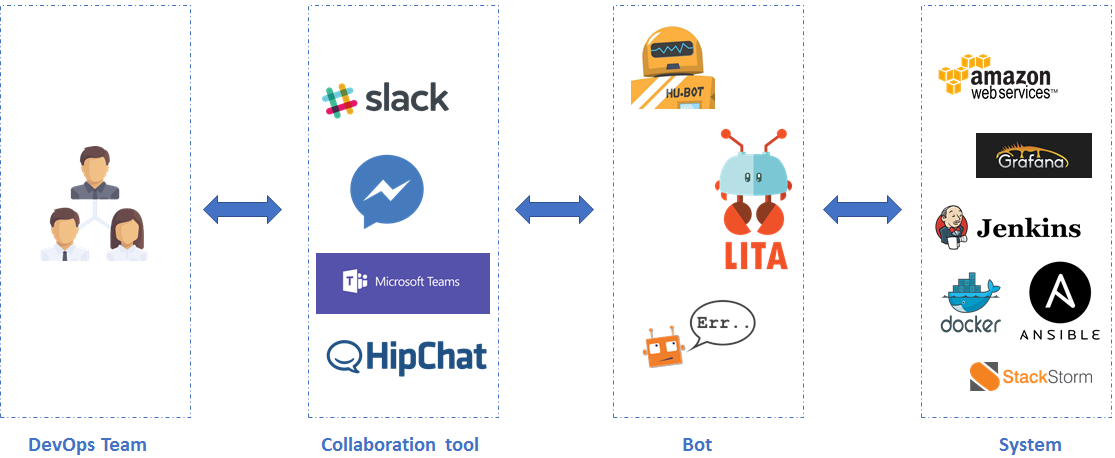
\includegraphics[width=\textwidth]{Anhang/cop}
  \quelle[o. \pno]{Zyane_2017_ChatOps}
  \caption{ChatOps Prozess}
\label{fig:cop}
\end{figure}


\subsubsection{Kollaborationswerkzeug}
Bekannte Beispiele für Kollaborationswerkzeuge sind Slack, Atlassian HipChat oder Cisco WebEx Teams, die allesamt die Integration von Bots ermöglichen.
Ziel solcher Werkzeuge ist es, Kollaboration zu ermöglichen, die Kommunikation von Arbeitsteams effektiv zu gestalten und klassische Kanäle wie E-Mail oder SMS abzulösen. Dabei ist auch die Anbindung von anderen Diensten, wie z. B. Cloud Speicher zur kollaborativen Bearbeitung von Dokumenten möglich. So müssen Unternehmen nicht zwangsläufig die Software von einem bestimmten Hersteller beziehen, sondern können das Kollaborationswerkzeug ihrer Wahl an verschiedene Dienste anbinden.
\footcites[Vgl.][o. \pno]{Zyane_2017_ChatOps}[Vgl.][o. \pno]{Koeltzsch_2019_Slack}

Slack zum Beispiel gilt als erfolgreichstes Kollaborationswerkzeug. Das Unternehmen wurde 2013 gegründet und hat heute 8 Millionen Nutzer, davon 3 Millionen zahlende und der Marktwert wird auf 7,1 Milliarden Dollar geschätzt. In der Basisversion ist es kostenlos, für Features wie längeres Vorhalten der Chatverläufe muss eine Lizenz erworben werden.
Zum Februar 2019 hat Slack den Konkurrenten HipChat abgeschaltet und die bisherigen Kunden nach Slack migriert, nachdem dieser Ende 2018 übernommen wurde.
\footcites[Vgl.][o. \pno]{Koeltzsch_2019_Slack}[Vgl.][o. \pno]{Donath_2018_Hipchat_Uebernahme}

\subsubsection{Bot}
Als ChatOps Bots können z. B. Hubot, Lita, oder  Errbot verwendet werden, wobei alle in etwa die gleiche Funktionalität besitzen, da sie sich am ursprünglichen ChatOps Bot Hubot orientieren.
Allerdings sind sie in verschiedenen Sprachen geschrieben, was für die Weiterentwicklung und Anbindung an Systeme wichtig sein kann, und weisen einige Besonderheiten auf. Eine Übersicht ist in \autoref{tab:bots} zu sehen.
\footcite[Vgl.][o. \pno]{Zyane_2017_ChatOps}

Cog hingegen ist ein Bot Framework, das möglichst plattformunabhängig arbeitet und ähnlich der Unix Funktion \textit{Pipe} funktioniert, also eine Verknüpfung verschiedener Befehle in beliebiger Komplexität ermöglicht.
\footcite[Vgl.][o. \pno]{Zyane_2017_ChatOps}

\begin{table}[H]
\centering
\begin{tabularx}{.8\textwidth}{l|l|X}
  Name & Sprache & Besonderheiten\\\hline
  Hubot & CoffeeScript & große Community\\
  Lita & Ruby & viele Plugins\\
  Errbot & Python & einfache Integration von APIs\\
  Cog & (Framework) & Unix-ähnliches Piping\\
\end{tabularx}
\quelleeigen[o. \pno]{Zyane_2017_ChatOps}
\caption{Verschiedene ChatOps Bots}
\label{tab:bots}
\end{table}

%\begin{table}[H]
%\centering
%\begin{tabularx}{1\textwidth}{|l|l|X|}\hline
%  Name & Sprache & Besonderheiten\\\hline\hline
%  Hubot & CoffeeScript & große Community\\\hline
%  Lita & Ruby & viele Plugins\\\hline
%  Errbot & Python & einfache Integration von APIs\\\hline
%  Cog & (Framework) & Unix-ähnliches Piping\\\hline
%\end{tabularx}
%\quelleeigen[o. \pno]{Zyane_2017_ChatOps}
%\caption{Verschiedene ChatOps Bots}
%\label{tab:bots}
%\end{table}

\subsubsection{Systemintegration}
Ein Chatbot kann z. B. an das Ticketsystem, Versionskontrollsystem, Konfigurationsmanagementsystem oder Monitoringsystem angebunden werden, um dort automatisiert Aufgaben auszuführen. Eine Auflistung mit Beispielen ist in \autoref{tab:integrations} zu finden.
\footcite[Vgl.][o. \pno]{Zyane_2017_ChatOps}

\begin{table}[H]
\centering
\begin{tabularx}{.8\textwidth}{l|X}
  System & Beispiele \\\hline
  Ticket& JIRA, OTRS, TeamForge \\
  Versionskontrolle & GitHub, GitLab, Bitbucket\\
  Konfigurationsmanagement & Ansible, Salt, Chef, Puppet\\
  Monitoring & Nagios, Check\_MK, Grafana, Prometheus, Kibana\\
  Continuous Integration & Jenkins, Travis CI, Bamboo\\
  \acf{IaC} & Docker, Swarm, Kubernetes, Terraform, Vagrant\\
\end{tabularx}
\quelleeigen[o. \pno]{Zyane_2017_ChatOps}
\caption{ChatOps Systemintegrationen}
\label{tab:integrations}
\end{table}

%\begin{table}[H]
%\centering
%\begin{tabularx}{1\textwidth}{|l|X|}\hline
%  System & Beispiele \\\hline\hline
%  Ticket& JIRA, OTRS, TeamForge \\\hline
%  Versionskontrolle & GitHub, GitLab, Bitbucket\\\hline
%  Konfigurationsmanagement & Ansible, Salt, Chef, Puppet\\\hline
%  Monitoring & Nagios, Check\_MK, Grafana, Prometheus, Kibana\\\hline
%  Continuous Integration & Jenkins, Travis CI, Bamboo\\\hline
%  \acf{IaC} & Docker, Swarm, Kubernetes, Terraform, Vagrant, Packer\\\hline
%\end{tabularx}
%\quelleeigen[o. \pno]{Zyane_2017_ChatOps}
%\caption{ChatOps Systemintegrationen}
%\label{tab:integrations}
%\end{table}

\section{CMDB}
Eine \acf{CMDB} ist ein aus dem \acf{ITIL} Umfeld stammendes Modell, um die IT-Infrastruktur eines Unternehmens abzubilden. Mit ihr kann auf Informationen zu Diensten und Konfigurationen zugegriffen werden.
\footcite[Vgl.][70\psq]{Olbrich_2008_ITIL}

Neben Hardware und Infrastruktur werden auch Dokumente wie Verträge, \acfp{SLA} oder Notfallpläne, sowie  Personen und Prozesse dort dokumentiert.
\footcite[Vgl.][253]{Sturm_2017_CMDB}


Die Komponenten einer \acs{CMDB} werden als \acfp{CI} bezeichnet. Ein \acf{CI} ist eine Einheit, die aus einem oder mehreren Objekten bestehen kann. Also z. B.~eine CPU, ein Kabel, ein kompletter Server, ein Netzwerksegment oder ein Cluster.
\footcite[Vgl.][70\psq]{Olbrich_2008_ITIL}

Zu den \acsp{CI} wird geplant, welchen Zweck diese erfüllen und in welchem Kontext sie eingesetzt werden (technisch und organisatorisch).
Es kann identifiziert werden, wer für das \acs{CI} zuständig ist und in welcher Version es vorliegt.
Sämtliche Änderungen an \acsp{CI} werden dokumentiert, wodurch eine vollständige Änderungshistorie über den gesamten Lebenszyklus entsteht.
\footcite[Vgl.][70\psq]{Olbrich_2008_ITIL}

Ein \acs{CI} kann verschiedene Eigenschaften bzw. Attribute besitzen und es können Verlinkungen zu anderen \acsp{CI} hergestellt werden, wodurch die Bildung einer Objekthierarchie möglich ist. Eine beispielhafte Anordnung ist in \autoref{fig:cih} zu sehen. \acsp{CI} werden außerdem in eine Kategorie eingeordnet und es kann ein Status zugewiesen werden.
\footcite[Vgl.][72\psqq]{Olbrich_2008_ITIL}

\begin{figure}[H]
  \centering
  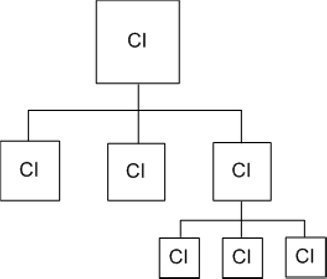
\includegraphics[width=0.3\textwidth]{Anhang/cih}
  \quelle[74]{Olbrich_2008_ITIL}
  \caption{Configuration Item Beziehungen}
\label{fig:cih}
\end{figure}


Neben rein hierarchischer Untergliederung sind auch andere Beziehungen zwischen \acsp{CI} möglich. Eine Übersicht mit Beispielen ist in \autoref{tab:bezci} zu sehen.\\
Durch die Verknüpfungen entsteht eine Übersicht, welche Systeme bei kritischen Ereignissen betroffen sind. Z. B.~welche Auswirkungen der Ausfall eines Switches hat.
\footcite[Vgl.][74\psq]{Olbrich_2008_ITIL}

\begin{table}[H]
\centering
\begin{tabularx}{0.8\textwidth}{l|X}
                            Beziehung & Beispiel \\\hline
                            X ist Teil von Y & eine CPU ist Teil eines Servers\\
                            X ist verbunden mit Y & ein Server ist mit einem Storagesystem verbunden \\
                            X benutzt Y & zwei Netzwerke benutzen eine VPN Verbindung \\
                            X ist eine Ausprägung von Y & gleicher Server, andere RAM Bestückung \\
\end{tabularx}
\quelleeigen[74]{Olbrich_2008_ITIL}
\caption{Beziehungen zwischen \aclp{CI}}
\label{tab:bezci}
\end{table}

%\begin{table}[H]
%\centering
%\begin{tabularx}{1\textwidth}{|l|X|}\hline
%                            Beziehung & Beispiel \\\hline\hline
%                            X ist Teil von Y & eine CPU ist Teil eines Servers\\\hline
%                            X ist verbunden mit Y & ein Server ist mit einem Storagesystem verbunden \\\hline
%                            X benutzt Y & zwei Netzwerke benutzen eine VPN Verbindung \\\hline
%                            X ist eine Ausprägung von Y & gleicher Server, andere RAM Bestückung \\\hline
%\end{tabularx}
%\quelleeigen[74]{Olbrich_2008_ITIL}
%\caption{Beziehungen zwischen \aclp{CI}}
%\label{tab:bezci}
%\end{table}


Jedes \acs{CI} durchläuft einen Lebenszyklus, der aus Beschaffung (Procurement), Betrieb (Operating) und Entsorgung (Disposal) besteht.
Die Beschaffung beinhaltet Bestellung und Lieferung. Sobald das \acs{CI} betriebsbereit ist, geht es in die Betriebsphase und wenn es ausgemustert wird, geht es in die Entsorgungsphase.\\
Je nach Phase können die \acsp{CI} verschiedene Zustände einnehmen. Diese können einen veränderbaren (V) oder finalen (F) Status haben. Eine Übersicht der Zustände pro Phase ist in \autoref{tab:statci} zu sehen.
\footcite[Vgl.][76\psq]{Olbrich_2008_ITIL}

\begin{table}[H]
\centering

\textit{Beschaffung}\\
\begin{tabularx}{.8\textwidth}{p{2cm}|c|X}
    Status      &  Art & Beschreibung                          \\\hline
    ordered     &  V & Bestellung wurde ausgelöst                 \\
    in progress &  V & Bestellvorgang wird bearbeitet             \\
    cancelled   &  F & Bestellung wurde storniert                 \\
    delivered   &  V & Ware wurde geliefert                       \\
    returned    &  F & Ware wurde zurückgesendet                  \\
\end{tabularx}

\bigskip\textit{Betrieb}\\
\begin{tabularx}{.8\textwidth}{p{2cm}|c|X}
    Status      &  Art & Beschreibung                          \\\hline
    active      &  V & CI ist im produktiven Einsatz              \\
    inactive    &  V & CI ist temporär nicht im Einsatz (Wartung) \\
    in store    &  V & CI ist im Lager                            \\
    planning    &  V & CI wird geplant                            \\
    test        &  V & CI wird getestet                           \\
\end{tabularx}

\bigskip\textit{Entsorgung}\\
\begin{tabularx}{.8\textwidth}{p{2cm}|c|X}
    Status      &  Art & Beschreibung                          \\\hline
    stolen      &  V & CI wurde gestohlen                         \\
    sold        &  F & CI wurde verkauft                          \\
    discarded   &  F & CI wurde ausgemustert                      \\
\end{tabularx}

\quelleeigen[77]{Olbrich_2008_ITIL}
\caption{Status von \aclp{CI}}
\label{tab:statci}
\end{table}


%\begin{table}[H]
%\centering
%
%\textit{Beschaffung}
%\begin{tabularx}{1\textwidth}{|p{2cm}|c|X|}\hline
%    Status      &  Art & Beschreibung                          \\\hline\hline
%    ordered     &  V & Bestellung wurde ausgelöst                 \\\hline
%    in progress &  V & Bestellvorgang wird bearbeitet             \\\hline
%    cancelled   &  F & Bestellung wurde storniert                 \\\hline
%    delivered   &  V & Ware wurde geliefert                       \\\hline
%    returned    &  F & Ware wurde zurückgesendet                  \\\hline
%\end{tabularx}
%
%\bigskip\textit{Betrieb}
%\begin{tabularx}{1\textwidth}{|p{2cm}|c|X|}\hline
%    Status      &  Art & Beschreibung                          \\\hline\hline
%    active      &  V & CI ist im produktiven Einsatz              \\\hline
%    inactive    &  V & CI ist temporär nicht im Einsatz (Wartung) \\\hline
%    in store    &  V & CI ist im Lager                            \\\hline
%    planning    &  V & CI wird geplant                            \\\hline
%    test        &  V & CI wird getestet                           \\\hline
%\end{tabularx}
%
%\bigskip\textit{Entsorgung}
%\begin{tabularx}{1\textwidth}{|p{2cm}|c|X|}\hline
%    Status      &  Art & Beschreibung                          \\\hline\hline
%    stolen      &  V & CI wurde gestohlen                         \\\hline
%    sold        &  F & CI wurde verkauft                          \\\hline
%    discarded   &  F & CI wurde ausgemustert                      \\\hline
%\end{tabularx}
%
%\quelleeigen[77]{Olbrich_2008_ITIL}
%\caption{Status von \aclp{CI}}
%\label{tab:statci}
%\end{table}


%\footcite[Vgl.][o. S.]{Drogseth_2015_CMDB}
%\footcite[Vgl.][o. S.]{Geissler_2018_CMDB}
%\footcite[Vgl.][o. S.]{Knittl_2010_CMDB}

% \footcite[Vgl.][o. S.]{itnovum_2013_cmdb}
% \footcite[Vgl.][o. S.]{Blokdijk_2008_CMDB}



\section{Python}
%\footcite[Vgl.][o. \pno]{Norton_2005_Python}
%\footcite[Vgl.][o. \pno]{Sumit_2019_Python_Chatbots}
Python ist eine universelle Programmiersprache, die auf vielen Betriebssystemen, wie Windows, Linux oder macOS läuft. Sie gilt als leicht zu erlernen und bietet objektorientierte Features. Sie wurde 1989 von Guido van Rossum als Nachfolger der Sprache \textit{ABC} entwickelt. Der Name ist angelehnt an die Fernsehsendung \textit{Monty Python's Flying Circus}.\\
Durch die \textit{batteries included} Philosophie sind viele Features schon in Python integriert.
\footcite[Vgl.][1\psqq]{Gowrishankar_2019_Python}

Um zusätzliche Module zu verwenden, wird empfohlen eine virtuelle Umgebung (\textit{virtualenv}) zu verwenden. So können Konflikte vermieden werden, wenn Tools Module in unterschiedlichen Versionen benötigen. Braucht z. B. ein Tool \textit{A} das Modul \textit{M} in der Version \textit{1.0} und ein Tool \textit{B} selbiges in der Version \textit{2.0}, so kann für jedes Tool ein eigenes \textit{virtualenv} angelegt werden. Auch Updates können in den Umgebungen getrennt von einander erfolgen.\\
Für gewöhnlich stellen Tools eine \textit{requirements.txt} Datei bereit, in der benötigte Module und deren Versionen vermerkt sind. Ein Beispiel ist in \autoref{requirements} zu finden.
\footcite[Vgl.][o. \pno]{Python_venv}

\begin{lstlisting}[language=python, label=requirements, caption=Beispiel requirements.txt]
novas==3.1.1.3
numpy==1.9.2
requests==2.7.0
\end{lstlisting}


\section{\acl{API}}
Eine \acs{API} ist eine Programmierschnittstelle, um Informationen auf standardisiertem Weg auszutauschen. Daten und Befehle werden strukturiert und in einer festgelegten Syntax übergeben.\\
Der Einsatz einer \acs{API} erlaubt die Modularisierung von Programmen, lediglich die Schnittstellen der Programmmodeule müssen spezifiziert sein. Außerdem bietet eine unveränderte \acs{API} eine hohe Stabilität auf lange Sicht, während der Quellcode darunter beliebig verändert werden kann.\\
Häufig verwendet werden werden APIs bei Online-Shops oder Content-Management-Systemen, z. B. um Bezahldienstleister, Bewertungssysteme oder Versanddienstleister anzubinden.
\footcite[Vgl.][o. \pno]{Luber_2017_API}

